\chapter{Style and Submission Requirements}\label{ch:style}

Requirements for other parts of the thesis work can be found on the thesis
Moodle page~\cite{Phu16}.  The requirements below are for the written thesis
only.

\section{Format}
The following format specifications must be adhered to for the thesis report
(the \LaTeX\ template available from the school ensures this):
\begin{enumerate}
\item The thesis must be typeset on \emph{A4 size page format} using a
legible \emph{\unit[12]{pt} font}.
\item The thesis must be prepared using a \emph{word-processor} of the
student's choice.
\item The thesis must be submitted electronically in
\emph{Portable Document Format} (pdf) with all \emph{fonts embedded}.
\item \emph{Margins} on all sides must be no less than \unit[25]{mm}.
\item \emph{1.5 line spacing} (about \unit[8]{mm} per line) must be used.
\item All pages must be \emph{numbered}. The main body of the thesis must be
numbered consecutively from beginning to end.  Other sections must either
be included or have their own logical numbering system.
\item The \emph{title page} must contain the following information:
\begin{enumerate}
\item University and School names.
\item Title of Thesis/Project.
\item Name of Author and student ID.
\item The degree the thesis is submitted for.
\item Submission date (month and year).
\item Supervisor's name.
\end{enumerate}
\end{enumerate}

\section{Other physical appearance}
Other requirements to the physical appearance of the thesis report are:
\begin{enumerate}
\item If a hardcopy is requested by supervisor or assessor, the report must be
\emph{printed} and \emph{spiral bound} (at the student's own cost).
\item Formulas must be \emph{typed} (not cut-and-pasted in).  Complicated or
difficult-to-type objects may be \emph{neatly
hand-drawn} and \emph{scanned in high resolution}.
\item \emph{Graphs, diagrams and photographs} should be inserted as close as
possible to their \emph{first reference} in the text. Rotated
graphs etc are to be arranged so as to be conveniently read, with the
bottom edge to the right-hand side of the page.
\emph{Graphs and diagrams must be legible!}
\item Relevant \emph{computer programs} and \emph{engineering drawings} should
be included in the thesis, usually in an appendix.
\end{enumerate}

\section{Submission}

Finally, here are some requirements to the submission procedure. 

\begin{enumerate}
\item All students are required to write and submit \emph{individual thesis
reports}.
The \emph{author} of the thesis is \emph{responsible} for the preparation of
the thesis, proofreading the
manuscript and having corrections made as necessary, and uploading the
thesis before the deadline.
\item A \emph{thesis summary sheet} must be included in the thesis report.
This summary sheet is designed to assist
in determining the overall input by students into the thesis work.
The guidelines for completing
the summary sheet and the summary sheet form can be downloaded from the
thesis Moodle site.
\item In some cases, the thesis work may involve \emph{several students}
working on a \emph{larger project}.
Thus, some aspects of the work may have been carried out
independently whilst other aspects may have been done as a group.  The
thesis reports must be \emph{clearly distinguishable}, and appropriately cross
referenced to each other.  The common work overlapping between the thesis
reports must be clearly identified.
\item There is a \emph{page limit} of 100 pages for the main body of the thesis.
\item If applicable, relevant data and program files should be put on a
\emph{CD-rom} and submitted directly to the thesis supervisor for archiving.
\end{enumerate}

%%%%%%%%%%%%%%%%%%%%%%%%%%%%%%%%%%%%%%%%%%%%%%%%%%%%%%%
%%%%%%%%%%%%%%%%%%%%%%%%%%%%%%%%%%%%%%%%%%%%%%%%%%%%%%%
%%%%%%%%%%%%%%%%%%%%%%%%%%%%%%%%%%%%%%%%%%%%%%%%%%%%%%%

\chapter{Content Requirements}\label{ch:content}

Students should consult the literature
(e.g.~\cite{Sid99,StrWhi79,Coo64,wrise16,Wol16})
and other resources for material on how to write a good
thesis.  The present document is only a very brief introduction as to what
is expected.

\nocite{NieLeh03,HasLehKwo05}

\section{Structure}
Most theses are structured similarly to the present document.
The main part of the thesis can be structured in many different ways,
however, but must contain: a \emph{problem definition}, \emph{scope}
and work \emph{motivation};
a contemporary \emph{literature review} on the thesis problem and relevant
related works;
relevant \emph{theory} and \emph{considerations} on how to solve the problem;
a description of the \emph{solution method} (dimensioning, construction,
etc.);
presentation of \emph{results} (measurements, simulations, etc.);
a \emph{discussion} of the results (validity, deviations, comparison
with previous solutions, etc.); and finally the \emph{conclusions}.

\section{Style of writing}

\begin{enumerate}

\item Audience:
The thesis must be addressed to engineers at the same level as the
student but without the special knowledge gained during the thesis work.
Such a third-person must be able to reconstruct the results on the basis
of the thesis alone.

\item
Every used concept/symbol/abbreviation which is not widely know must be \emph{defined}.
The wording should be \emph{short} and \emph{concise};  a suitable length
is 40--70 pages (plus appendices).
Readable(!) \emph{figures} and \emph{graphs} enhance comprehensibility.

\item Units.
\emph{SI units} must be used.  Units must be used correctly throughout the
thesis.
\end{enumerate}

\section{Documentation}

\begin{enumerate}
\item
The work must be well documented; i.e. enclosed must be the \emph{complete
schematics} of designed electronic circuits/test set-ups and/or a
\emph{program listing}, and/or etc.
Documentation of \emph{simulation results} and/or \emph{measurement
results} likewise.
\item References:
For every declaration/equation/method/etc., which is not widely known,
a \emph{reference to the literature} must be given (or a `proof' if it is
the authors own work).
In case material is copied verbatim, quotes and references must be used.
This is also the case when referring to partners
work in larger projects.  Figures not of the student's own making must have
the source referenced in the figure caption.

\item Plagiarism:
Failure to give proper references to the literature is \emph{plagiarism}.
Plagiarism is considered serious offence and severe penalties may apply.

\end{enumerate}

\section{Avoiding common problems}

The thesis project, including the thesis report, is expected to be a
professionally executed body work.  Solutions to some commonly seen report
problems are given below.

\subsection{Figure quality}
If at all possible, students should create their own figures using
suitable software packages, as shown in the example
in Figure~\ref{fig-schematic}.  It is possible to use bitmap figures (as
opposed to vector graphics) that are not photographs, but it must be ensured
that the resolution is high
and that lines and text are clear and have good contrast.
Legibility is key: the pdf files generated from the used
word processor should be verified for legibility early.

\begin{figure}[ht!]
\centering
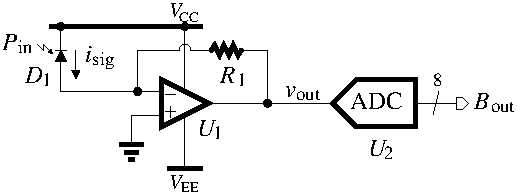
\includegraphics{schematic}
\caption{Schematic of electronic circuit.}
\label{fig-schematic}
\end{figure}

When graphs are including in the thesis, again it must be ensured that the
plotting software generates clear, legible outputs and that axes have
clear labels as shown in Figure~\ref{fig-plot}.

\begin{figure}[ht!]
\centering
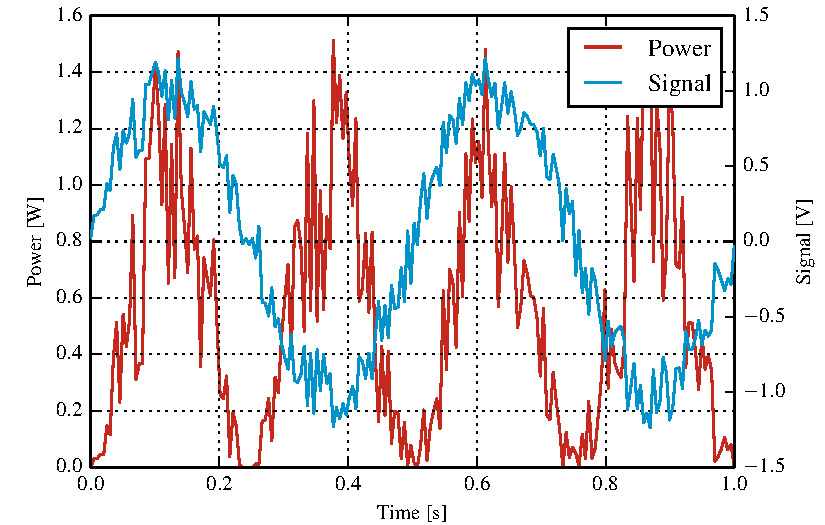
\includegraphics{plotout}
\caption{Plot of some random data.}
\label{fig-plot}
\end{figure}

\subsection{Attention to detail}

It is key to a good document that the author pays attention to detail.  This
includes concise definitions and descriptions, making sure that concepts are
explained in a logical order that the reader can follow, and that consistent
symbol use is diligently practiced.  For instance: ``the output voltage,
$v_{\rm out}$ in Figure~\ref{fig-schematic} is given by
Equation~\ref{eq-vout}, where it is assumed that $R_1=\unit[1]{k\Omega}$''. 

\begin{equation}
v_{\rm out}=-R_1\cdot i_{\rm sig}
\label{eq-vout}
\end{equation}

\subsection{Story telling}
It is important that the reader knows where the writing in thesis is heading
at all times.  An early introduction of high-level conceptual design of the
proposed solution can be a good help, as can a well defined thesis scope.
Developing well-constructed, logical arguments for the work also greatly
help in convincing the reader of the thesis merits.
